\section{Spheres}
Let's add a new object: a sphere. The same kind of computations must be applied to a triangle and a sphere. Both are 3D objects, they have a reflectance $\rho$, are made of a specific material (only diffuse for now), have a normal and must be able to compute their intersection with a ray.

Where a triangle is described by its 3 vertices, a sphere has a center C(cx, cy, cz) and a radius R. The intersection between a sphere and a ray is explained below, with P(px, py, pz) the starting point of the ray, $\vec{v}$ the ray direction and I the intersection.

$dx = \vec{v}.x$

$dy = \vec{v}.y$

$dz = \vec{v}.z$

$a = dx^2 + dy^2 + dz^2$

$b = 2 dx (px - cx) + 2 dy (py - cy) + 2 dz (pz - cz)$

$c =  cx^2 + cy^2 + cz^2 + px^2 + py^2 + pz^2 - 2 (cx * pc + cy * py + cz * pz) - R^2$

The discriminant is $d = b^2 - 4 a c$

If $d < 0$ there is no intersection, if $d = 0$ the ray is tangent to the sphere and intersects it in one point, if $d > 0$ the ray intersects the sphere in two points.

To compute the closest intersection, solve our equation by computing m, $m = \frac{-b -\sqrt{d}}{2a}$

This value represents the number of times $\vec{v}$ must be added to P to reach the closest intersection I.

Therefore, I(ix, iy, iz) is

$ix = px + t dx$

$iy = py + t dy$

$iz = pz + t dz$\\


Now that we have our intersections, we must still compute the normal $\vec{n}$ at the intersection to obtain the amount of light reaching our intersection. The normal direction depends on the relative position between the intersection and the center of the sphere. Therefore,

\begin{equation}
\vec{n} = \frac{I - C}{R}
\end{equation}

\begin{figure}[H]
\centering
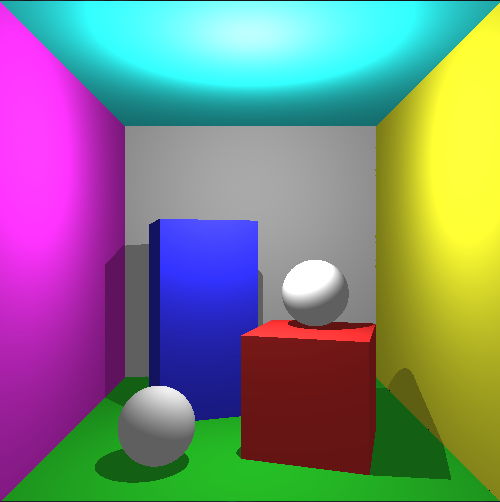
\includegraphics[width=0.4\linewidth]{img/spheres.jpg}
\caption{Spheres (930 ms)}
\end{figure}


\section{Ray-triangle intersection: optimization}
The intersection algorithm is the core of our raytracer and the most called method in our entire program. It is also a bottleneck which could be optimized and lead to great performances.

By trying to reduce the render time of the ray tracer, I found an interesting paper describing a fast ray-triangle intersection algorithm by T. Möller and B. Trumbore \cite{moller2005fast}.

While the algebra used for the calculations is slightly more complex than our previous algorithm, this implementation happens to be way faster, and reduced the render time of the overall process by 2.6 times. Our scene is now rendered in 360 ms instead of 930 ms.


\section{Specular materials}
The performances have been improved but our scene could be better. An interesting effect, which can also be very costly, would be to add specular materials.

The way to do so is quite simple. Previously, the color of a pixel was obtained by multiplying the reflectance of the intersected object to the power light hitting the area, plus the indirect light constant. This procedure won't change, but we now check the material of the intersected object. If it's a specular material, we trace a new ray from the intersection and the color of the pixel will be the one hit by the new ray.

The direction of the new ray is described in equation \ref{eq:specular}, where $\vec{d_i}$ is the incident ray direction, $\vec{n}$ the normal at the intersection and $\vec{d_r}$ the reflected ray direction.

\begin{equation}
\vec{d_r} = \vec{d_i} - 2 (\vec{n} \cdot \vec{d_i}) \vec{n}
\label{eq:specular}
\end{equation}

This operation can be costly if we have many bounces between two specular materials, but it will also give a very nice visual effect. To prevent infinite bounces, we must however limit the maximal number of bounces, and return a default value when this threshold is reached. In the figure below, we can observe the multiple bounces with the left purple wall rendered in the mirror of the tall blue box after a bounce on the specular sphere. The black color reflected is the default color assigned to the "void", i.e. when a ray don't hit any object.

\begin{figure}[H]
\centering
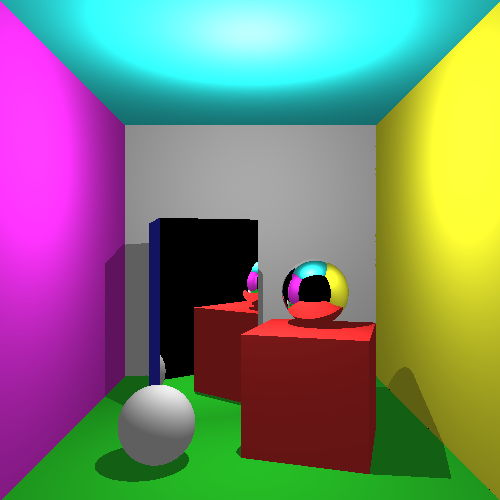
\includegraphics[width=0.35\linewidth]{img/specular.jpg}
\caption{Specular materials}
\end{figure}


\section{Glass - Refraction}
Glass is another interesting material. Yet, this one is tricky since is should refract and reflect rays, each ray having its own percentage of light transmitted according to the incident ray angle. In a first step, we will only implement refraction.

The refraction and reflection formulas to compute those directions and percentages are described in by T Whitted in \cite{whitted1979improved}. However, a faster method, which can actually be proven as equivalent to the previous one using trigonometry and vector algebra, is detailed by PS Heckbert in \cite{heckbert1989derivation}.

The idea lying in those papers is to first compute the cosine angle between the incident vector and the normal at the intersection.

$ cos\theta_1 = \vec{d_i} \cdot \vec{n} $

If the cosine is higher than 0, the incident and normal vectors have the same direction. If so, this means that we are inside the material, so we have already performed a refraction and want to perform a second one. We must therefore use $-\vec{n}$ instead of $\vec{n}$ to compute the next ray direction.

We respectively define $i_1$ and $i_2$ the refractive indices of the current and next material. We remind that $i_{air} \approx 1.0$ and $i_{glass} \approx 1.52$ for most glass materials (nice effects can be obtained by using crystal and caustics, but this feature has not been implemented here).

$\eta = \frac{i_1}{i_2}$

\begin{equation}
cos2\theta_1 = 1 - \eta^2 (1 - cos\theta_1^2)
\label{eq:refraction_percent}
\end{equation}

If $cos2\theta_1$ is lower than 0, the incident ray is completely reflected. This effect, happening when the angle between the incident ray and the normal is higher than a certain threshold, is called \textit{total internal reflection}. $cos2\theta_1$ can actually be approximated as the percentage of light refracted. This is a very useful measure.

The reflected ray direction is then calculated in the same way as in equation \ref{eq:specular}. The refracted ray direction is details in equation \ref{eq:refracted_angle} where $d_R$ is the refracted ray direction.

\begin{equation}
\vec{d_R} = \eta \vec{d_i} + (\eta cos\theta_1 - \sqrt{cos2\theta_1}) \vec{n}
\label{eq:refracted_angle}
\end{equation}

\begin{figure}[H]
\centering
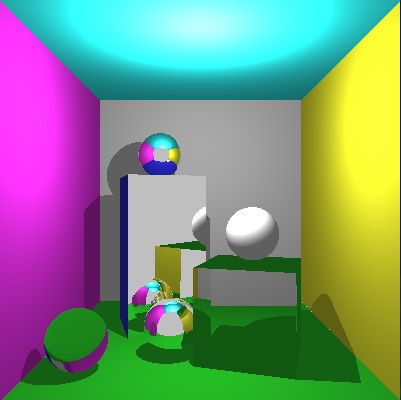
\includegraphics[width=0.35\linewidth]{img/glass_refraction.jpg}
\caption{Refraction through glass (430 ms)}
\label{fig:glass_refraction}
\end{figure}

As specified before, the reflection is not rendered in the previous figure. However, we can observe a total internal reflection with the yellow wall reflected in the mirror after multiple bounces in the glass. Yet, if most of the light should be reflected by the top of the box due to the incident angle, we haven't applied yet the percentage to the refracted ray, which explains the green color.

The smoked glass effect is obtained by reducing the refracted light transmitted by 5\% when entering the object.


\section{Anti-aliasing}
Our scene looks better now. Though the geometry could be improved. Many artifacts could be observed on the edges of figure \ref{fig:glass_refraction}. This aliasing is quite annoying, let's fix it. The following describes various anti-aliasing methods supported by the raytracer. Those algorithms are applied in post-processing, i.e. after the scene has been generated.

\subsection{Edges detection}
Since anti-aliasing can be a costly operation, we want to target only the pixels on the edges, this will avoid an important waste of time.

Instead of displaying a pixel immediately after its computation, we store them in a 2D matrix representing our screen and containing the RGB vector of each pixel. When our scene is complete, we transform this matrix in a grayscale matrix containing values from 0 to 255 instead of RGB vectors. The transformation in equation \ref{eq:grayscale} respects the CCIR 601 recommendations. $I$ is the grayscale intensity, and $\vec{rgb}$ a RGB vector. Figure \ref{fig:grayscale} is the output of this transformation.

\begin{equation}
I = \vec{rgb} \cdot (0.2989, 0.5870, 0.1140)
\label{eq:grayscale}
\end{equation}

Once we have computed the intensity, we must detect the intensity variations in the scene. This is achieved using the Sobel operator \cite{sobel19683x3}. We define $p_1$ ... $p_9$ the nine values constituting a 3x3 matrix, where $p_1$ is above and to the left, $p_5$ is the pixel itself, and $p_9$ is below and to the right. If the result of equation \ref{eq:sobel} is higher than a threshold (here 0.5), we add the pixel coordinates to a list on which anti-aliasing must be applied. Those pixels are displayed in white in figure \ref{fig:sobel}

\begin{equation}
 g = |( p_1 + 2 * p_2 + p_3 ) - ( p_7 + 2 * p_8 + p_9 )| + |( p_3 + 2 * p_6 + p_9 ) - ( p_1 + 2 * p_4 + p_7 )|
\label{eq:sobel}
\end{equation}

\begin{figure}[H]
\centering
\minipage[t]{0.4\textwidth}
    \centering
    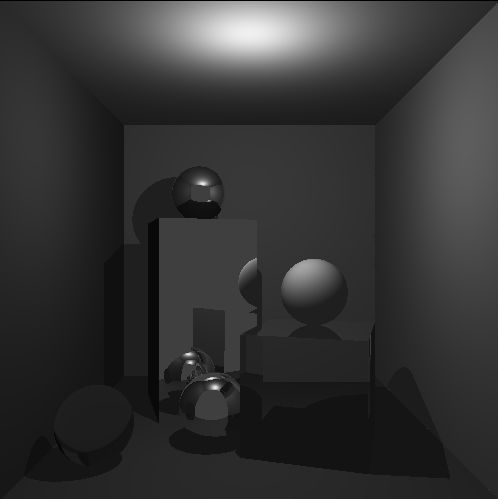
\includegraphics[width=\linewidth]{img/antialiasing/grayscale.jpg}
    \caption{Grayscale scene}
    \label{fig:grayscale}
\endminipage
\minipage[t]{0.4\textwidth}
    \centering
    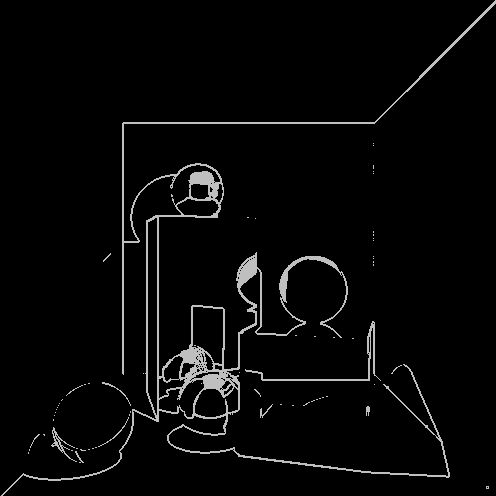
\includegraphics[width=\linewidth]{img/antialiasing/sobel.jpg}
    \caption{Edges detection (Sobel operator)}
    \label{fig:sobel}
\endminipage
\end{figure}


\subsection{Uniform}
Once we know which pixels need anti-aliasing, we can improve the accuracy of our edges by shooting multiple rays in various directions inside each pixel.

\begin{figure}[H]
\centering
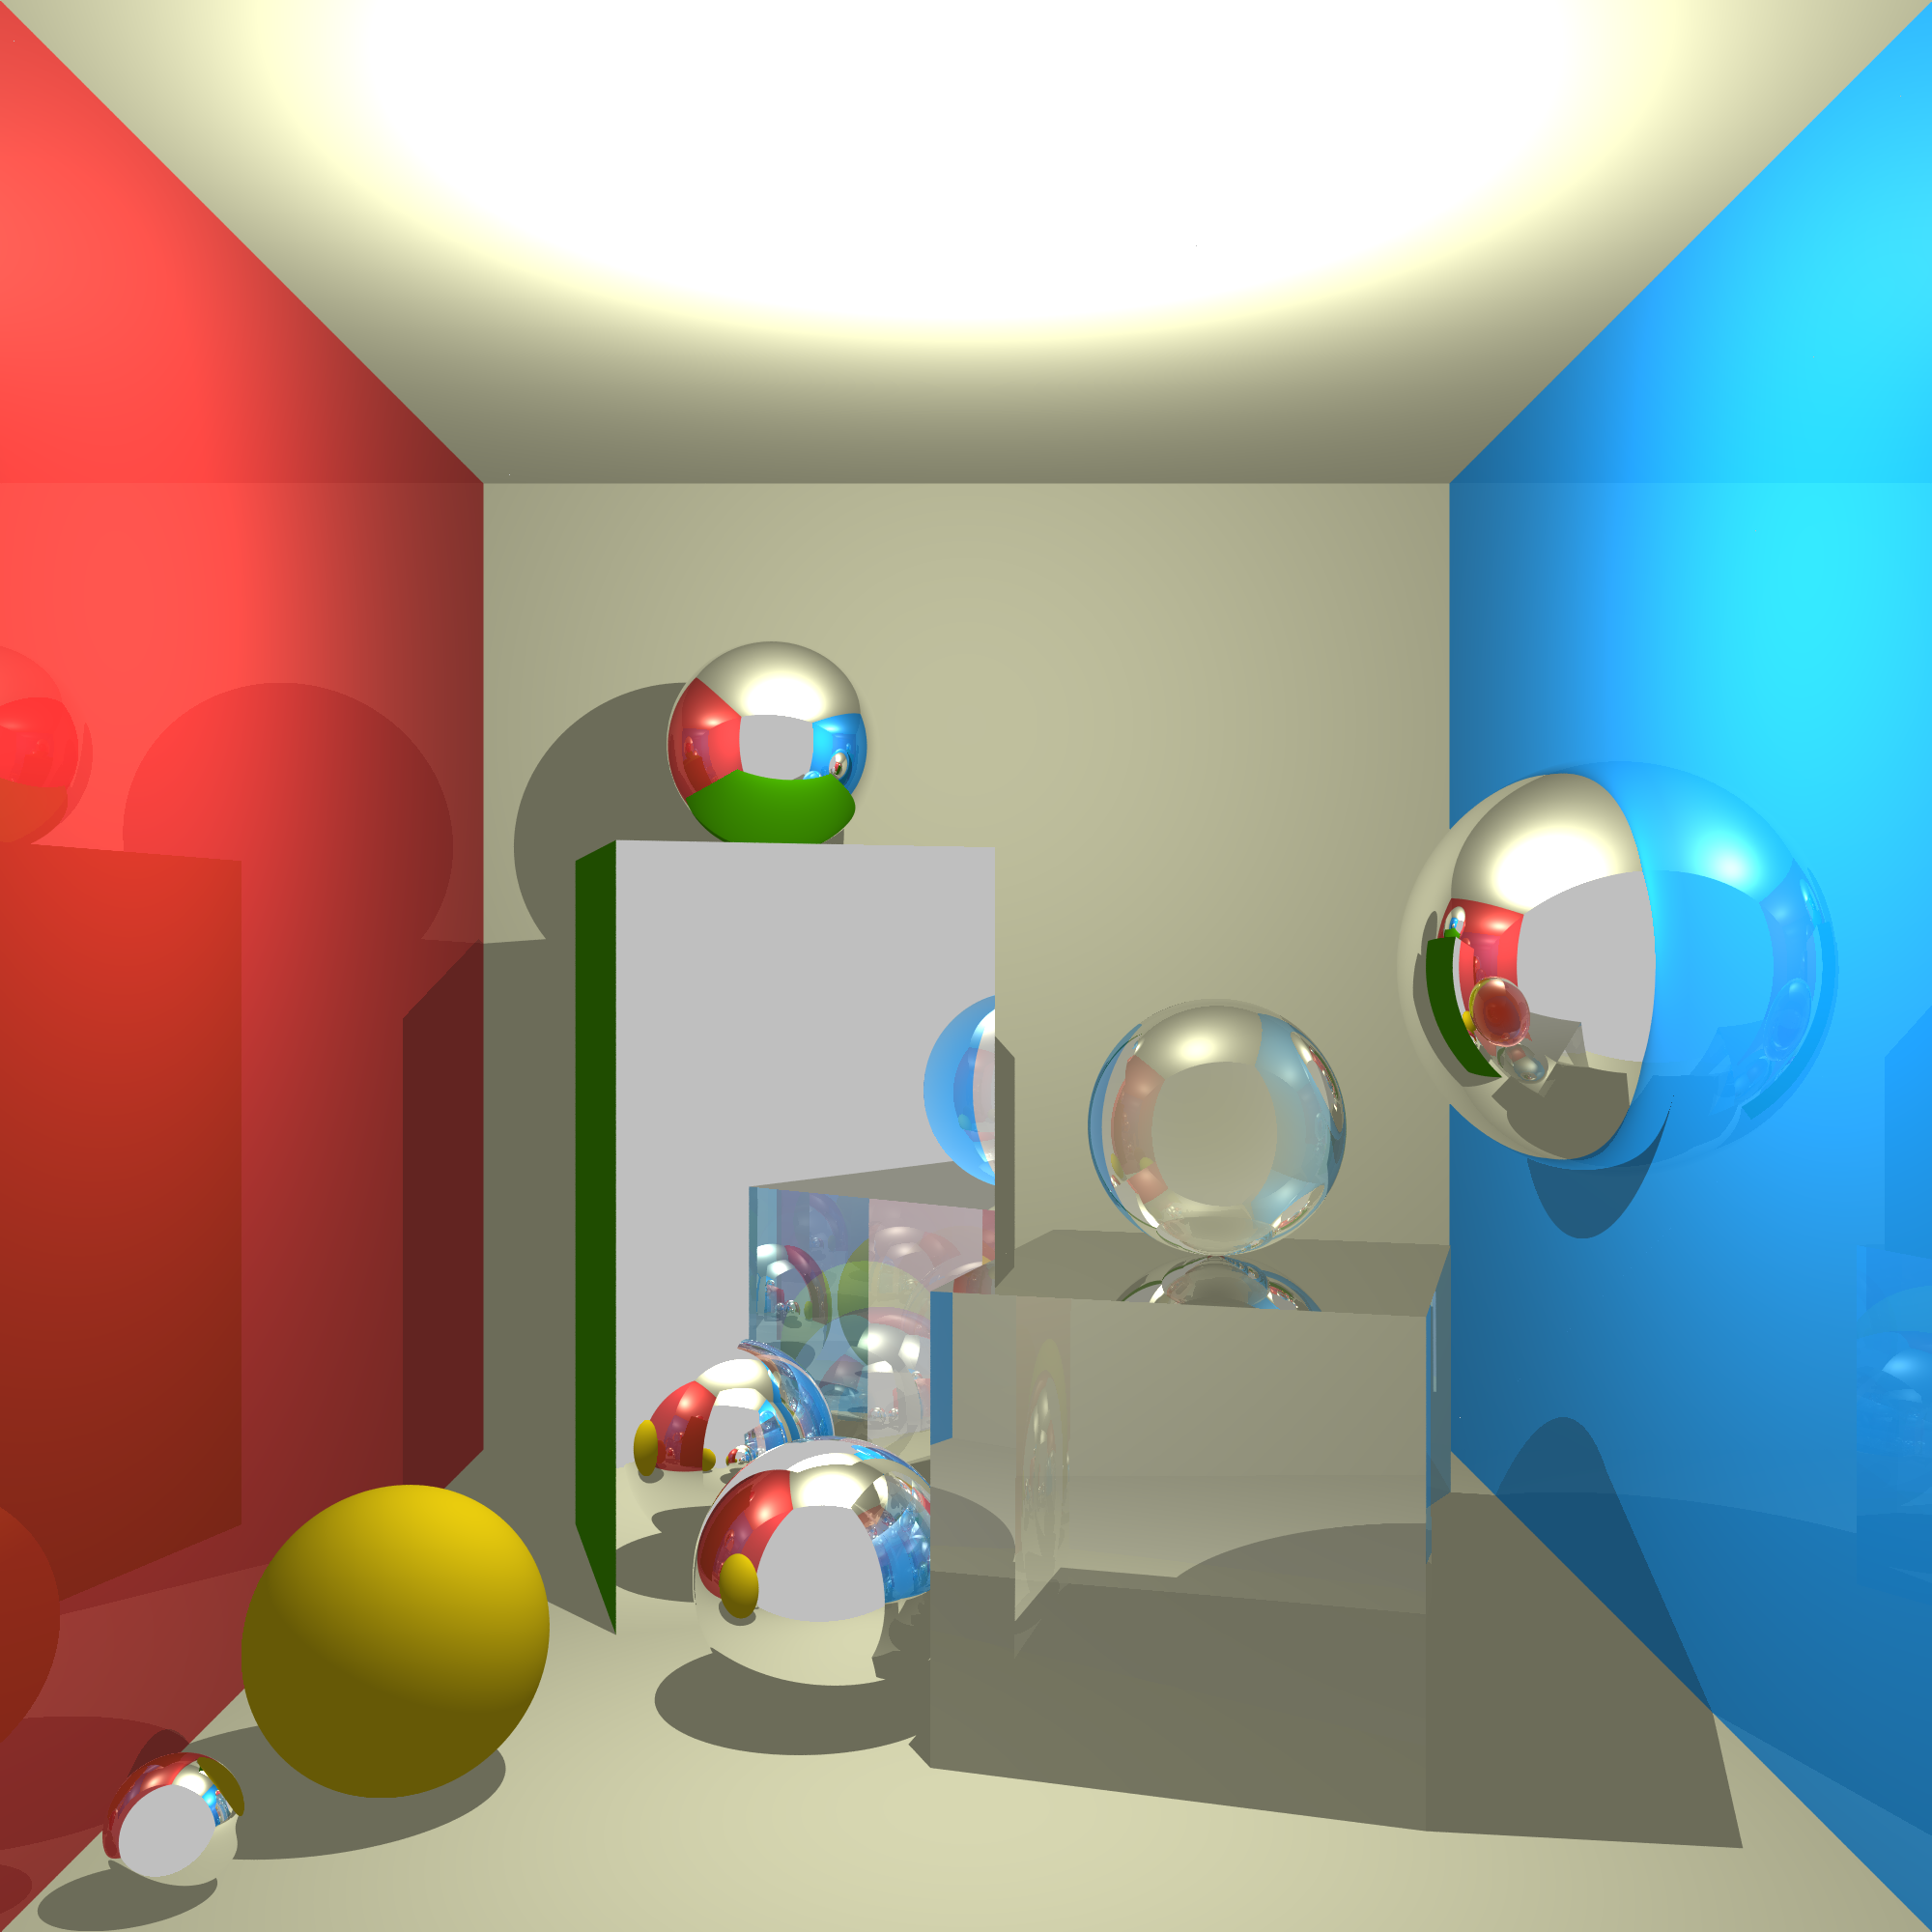
\includegraphics[width=0.35\linewidth]{img/glass_awesome.png}
\caption{Uniform anti-aliasing 8x}
\end{figure}

\subsection{Stochastic sampling}

They are zoomed
\begin{figure}[H]
\minipage{0.25\textwidth}
    \centering
    
\includegraphics[width=\linewidth]{img/antialiasing/no_aa.png}
    \caption{AA disabled (430 ms)}
\endminipage\hfill
\minipage{0.25\textwidth}
    \centering
    
\includegraphics[width=\linewidth]{img/antialiasing/super8x.png}
    \caption{Uniform 8x (1200 ms)}
\endminipage\hfill
\minipage{0.25\textwidth}
    \centering
    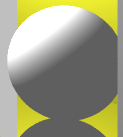
\includegraphics[width=\linewidth]{img/antialiasing/sto8x.png}
    \caption{Jittered 8x (1250 ms)}
\endminipage\hfill
\minipage{0.25\textwidth}
    \centering
    
\includegraphics[width=\linewidth]{img/antialiasing/sto16x.png}
    \caption{Jittered 16x (1450 ms)}
\endminipage\hfill
\end{figure}


\begin{figure}[H]
\centering
\minipage[t]{0.4\textwidth}
    \centering
    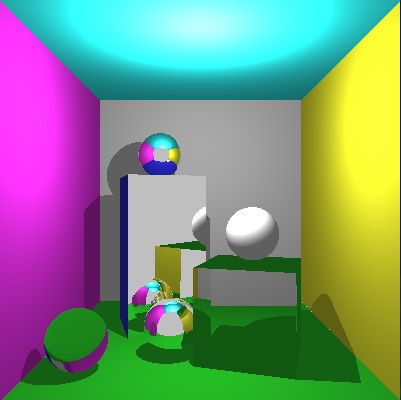
\includegraphics[width=\linewidth]{img/glass_refraction.jpg}
    \caption{Anti-aliasing disabled (430 ms)}
\endminipage
\minipage[t]{0.4\textwidth}
    \centering
    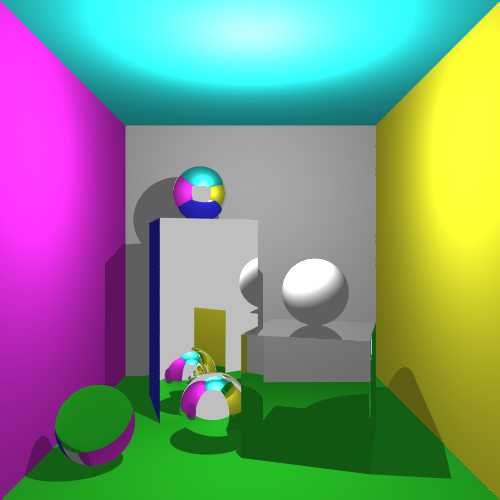
\includegraphics[width=\linewidth]{img/antialiasing/stoAA16x_full.png}
    \caption{Stochastic sampling 16x (1450 ms)}
\endminipage
\end{figure}


\section{Glass - Reflection}
20 bounces, remove smoked glass
\begin{figure}[H]
\centering
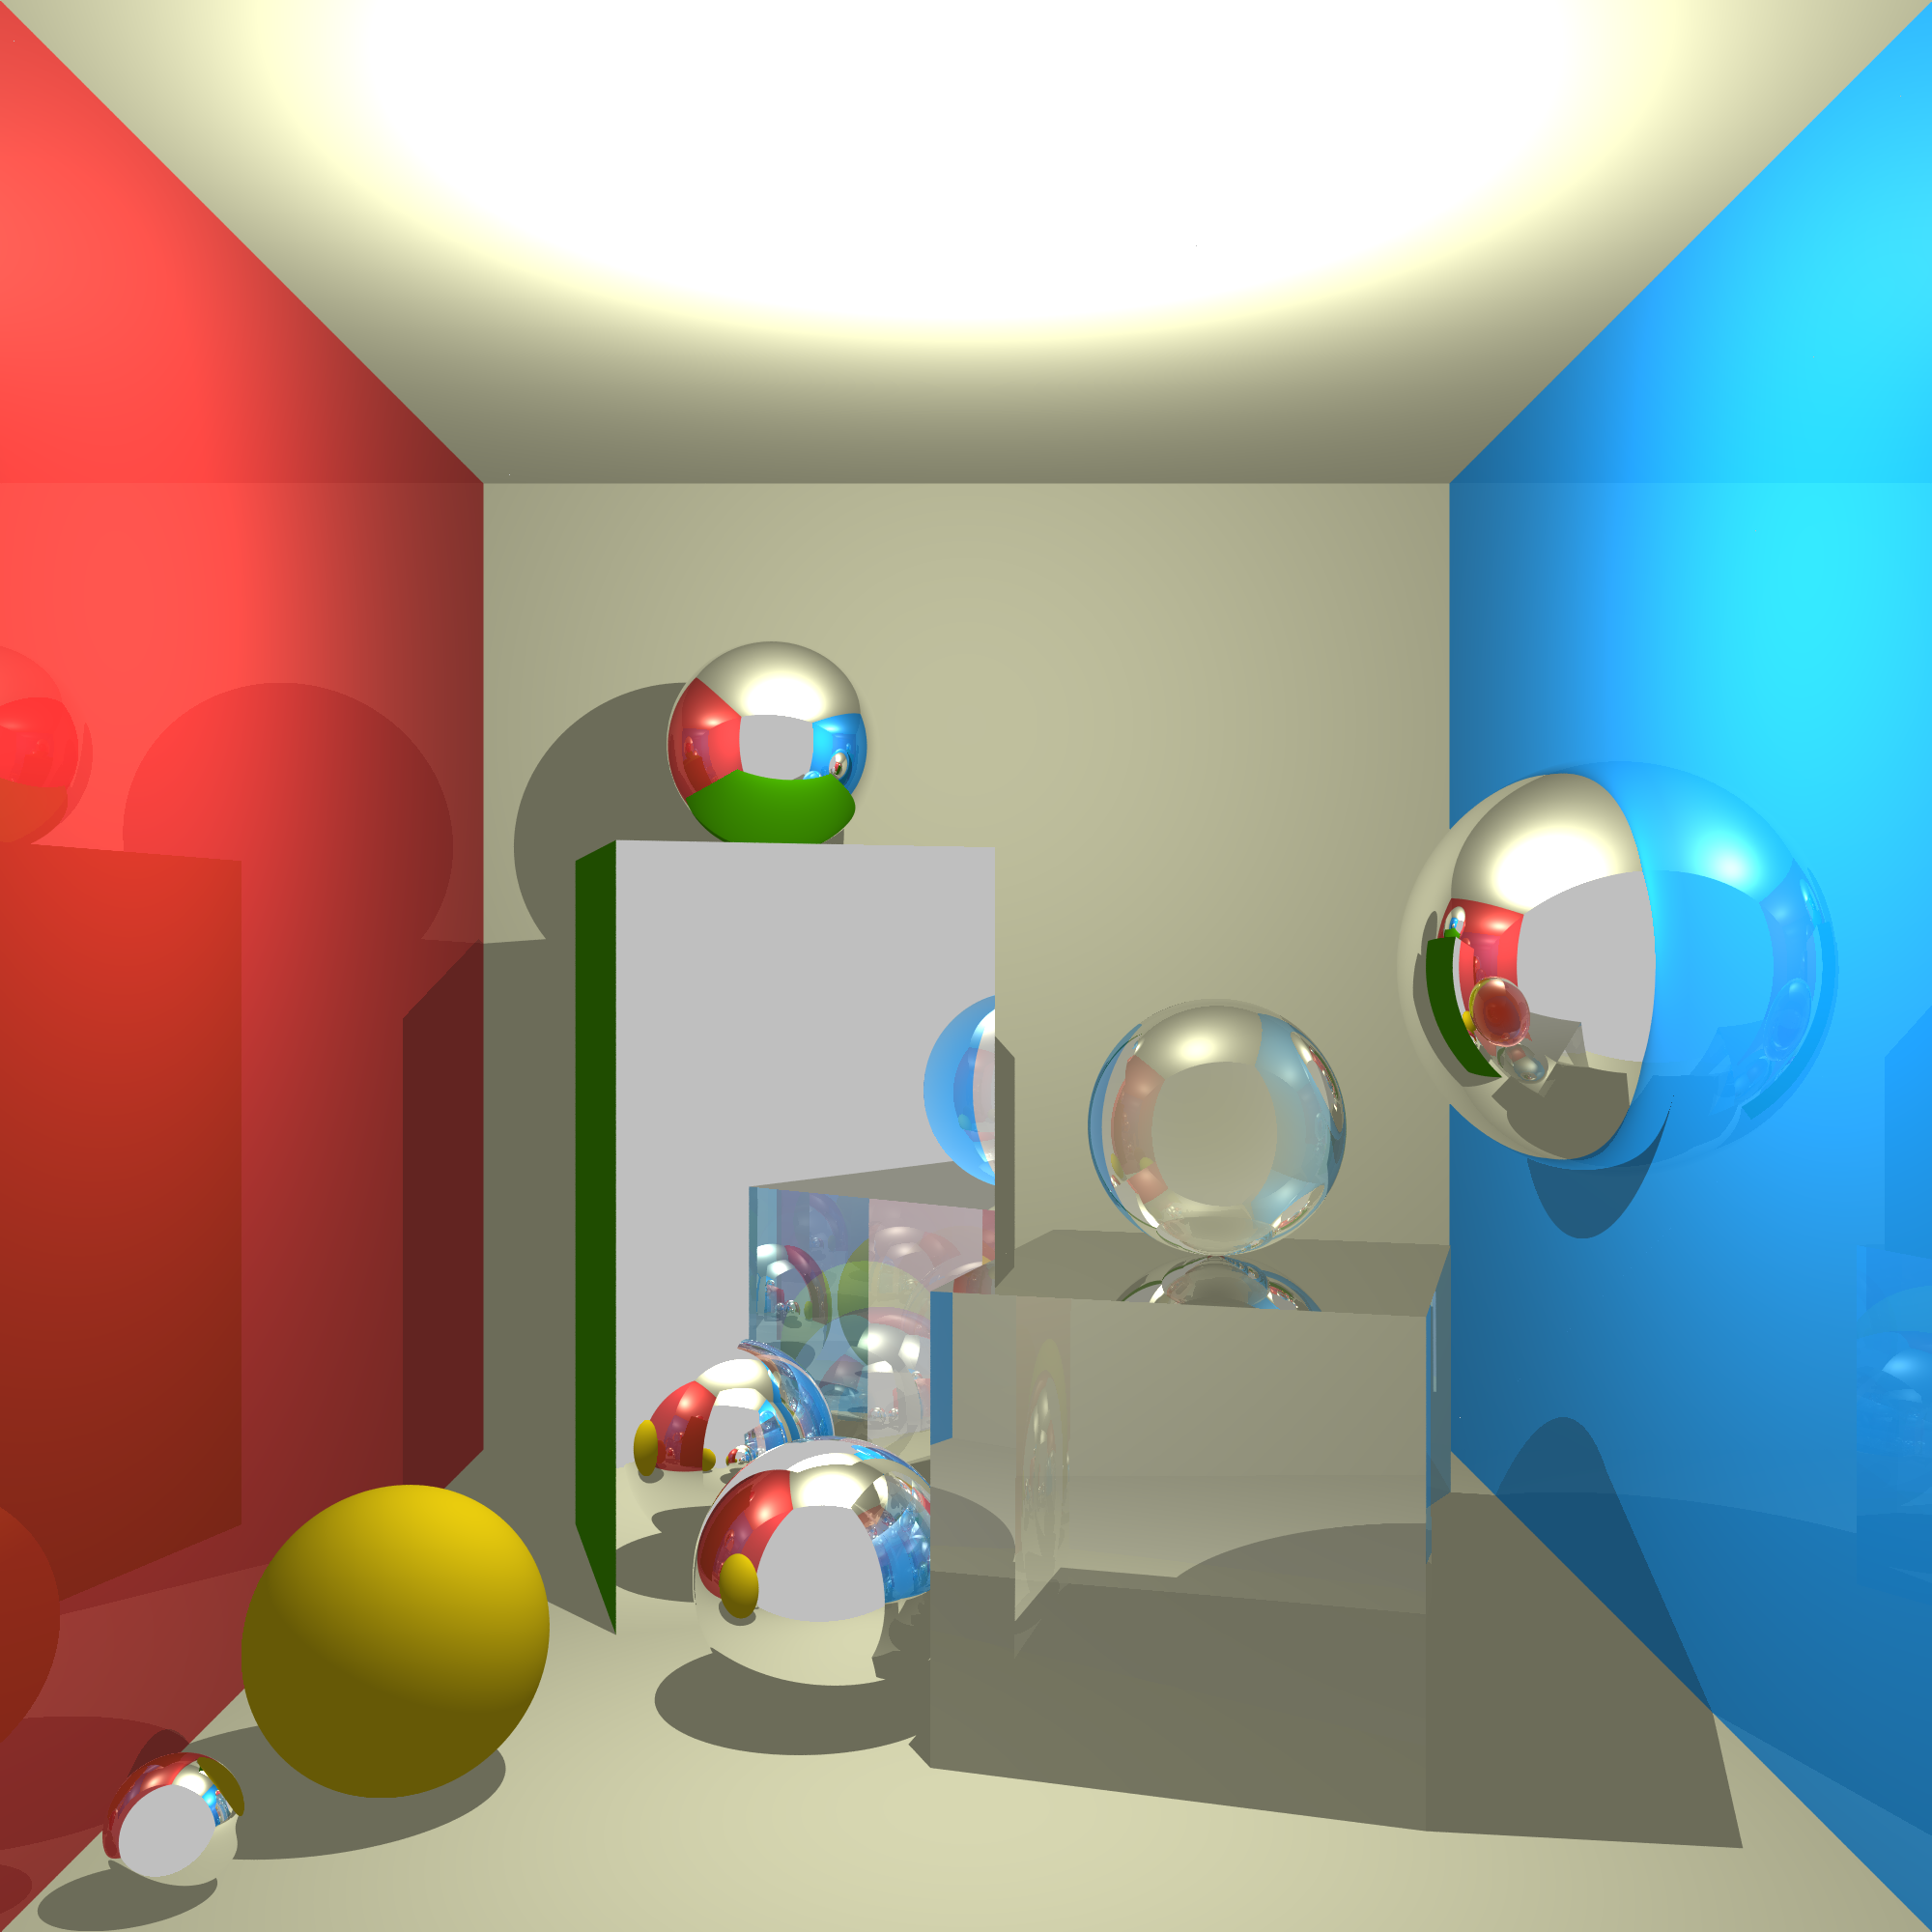
\includegraphics[width=0.35\linewidth]{img/glass_awesome.png}
\caption{Glass: refraction and reflection}
\end{figure}


\section{Soft shadows}
\subsection{Uniform light sources}
The following scenes were processed for a 500x500 resolution without anti-aliasing.
\begin{figure}[H]
\minipage{0.33\textwidth}
    \centering
    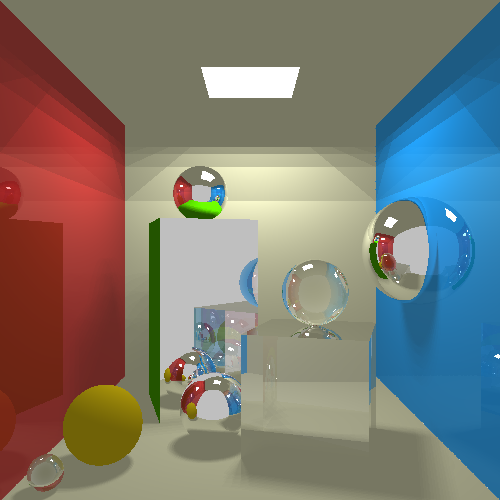
\includegraphics[width=\linewidth]{img/shadows/16.png}
    \caption{16 lights, uniform (8700 ms)}
\endminipage\hfill
\minipage{0.33\textwidth}
    \centering
    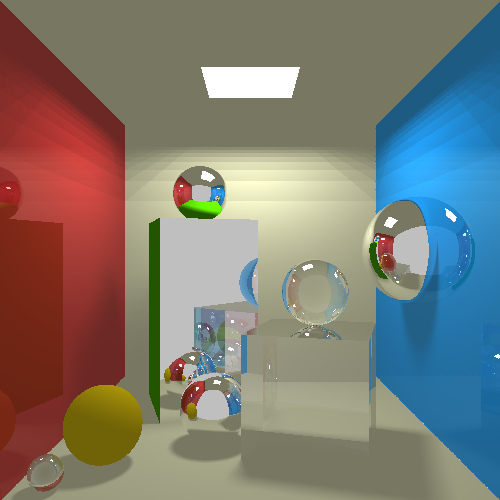
\includegraphics[width=\linewidth]{img/shadows/64.png}
    \caption{64 lights, uniform (30 600 ms)}
\endminipage\hfill
\minipage{0.33\textwidth}
    \centering
    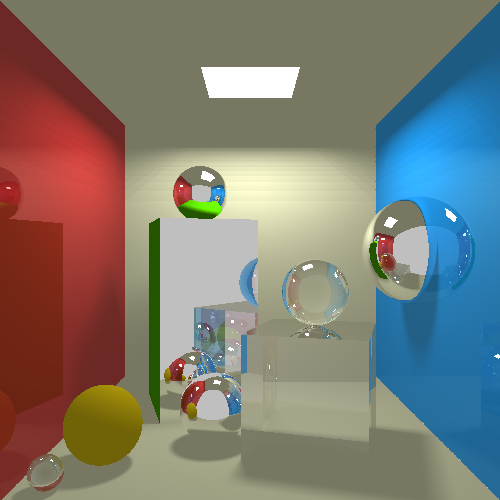
\includegraphics[width=\linewidth]{img/shadows/256.png}
    \caption{256 lights, uniform (118 500 ms)}
\endminipage\hfill
\end{figure}

\subsection{Jittered light sources}
\begin{figure}[H]
\minipage{0.33\textwidth}
    \centering
    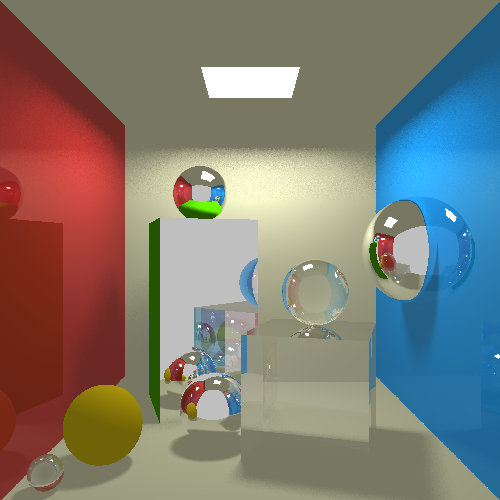
\includegraphics[width=\linewidth]{img/shadows/16_jittered.png}
    \caption{16 lights, jittered (9400 ms)}
\endminipage\hfill
\minipage{0.33\textwidth}
    \centering
    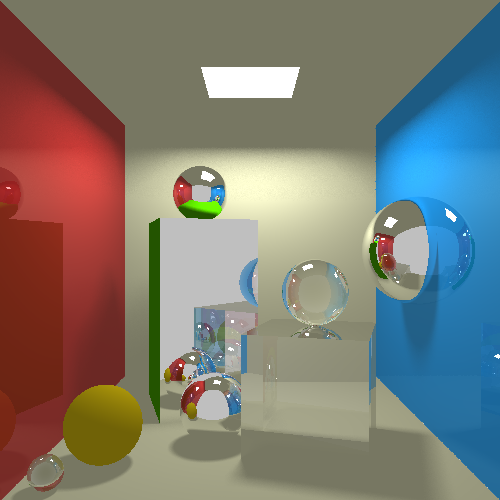
\includegraphics[width=\linewidth]{img/shadows/64_jittered.png}
    \caption{64 lights, jittered (33 600 ms)}
\endminipage\hfill
\minipage{0.33\textwidth}
    \centering
    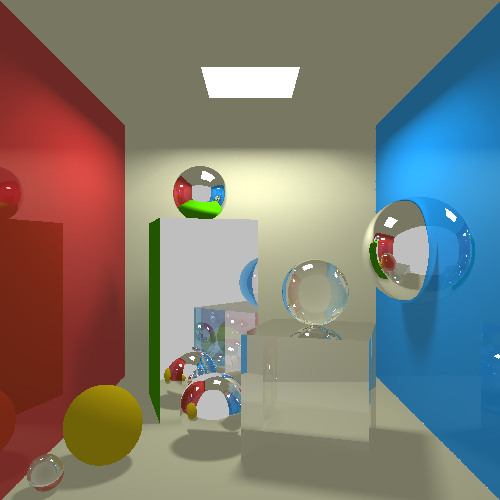
\includegraphics[width=\linewidth]{img/shadows/256_jittered.png}
    \caption{256 lights, jittered (128 600 ms)}
\endminipage\hfill
\end{figure}

%\begin{figure}[H]
%\centering
%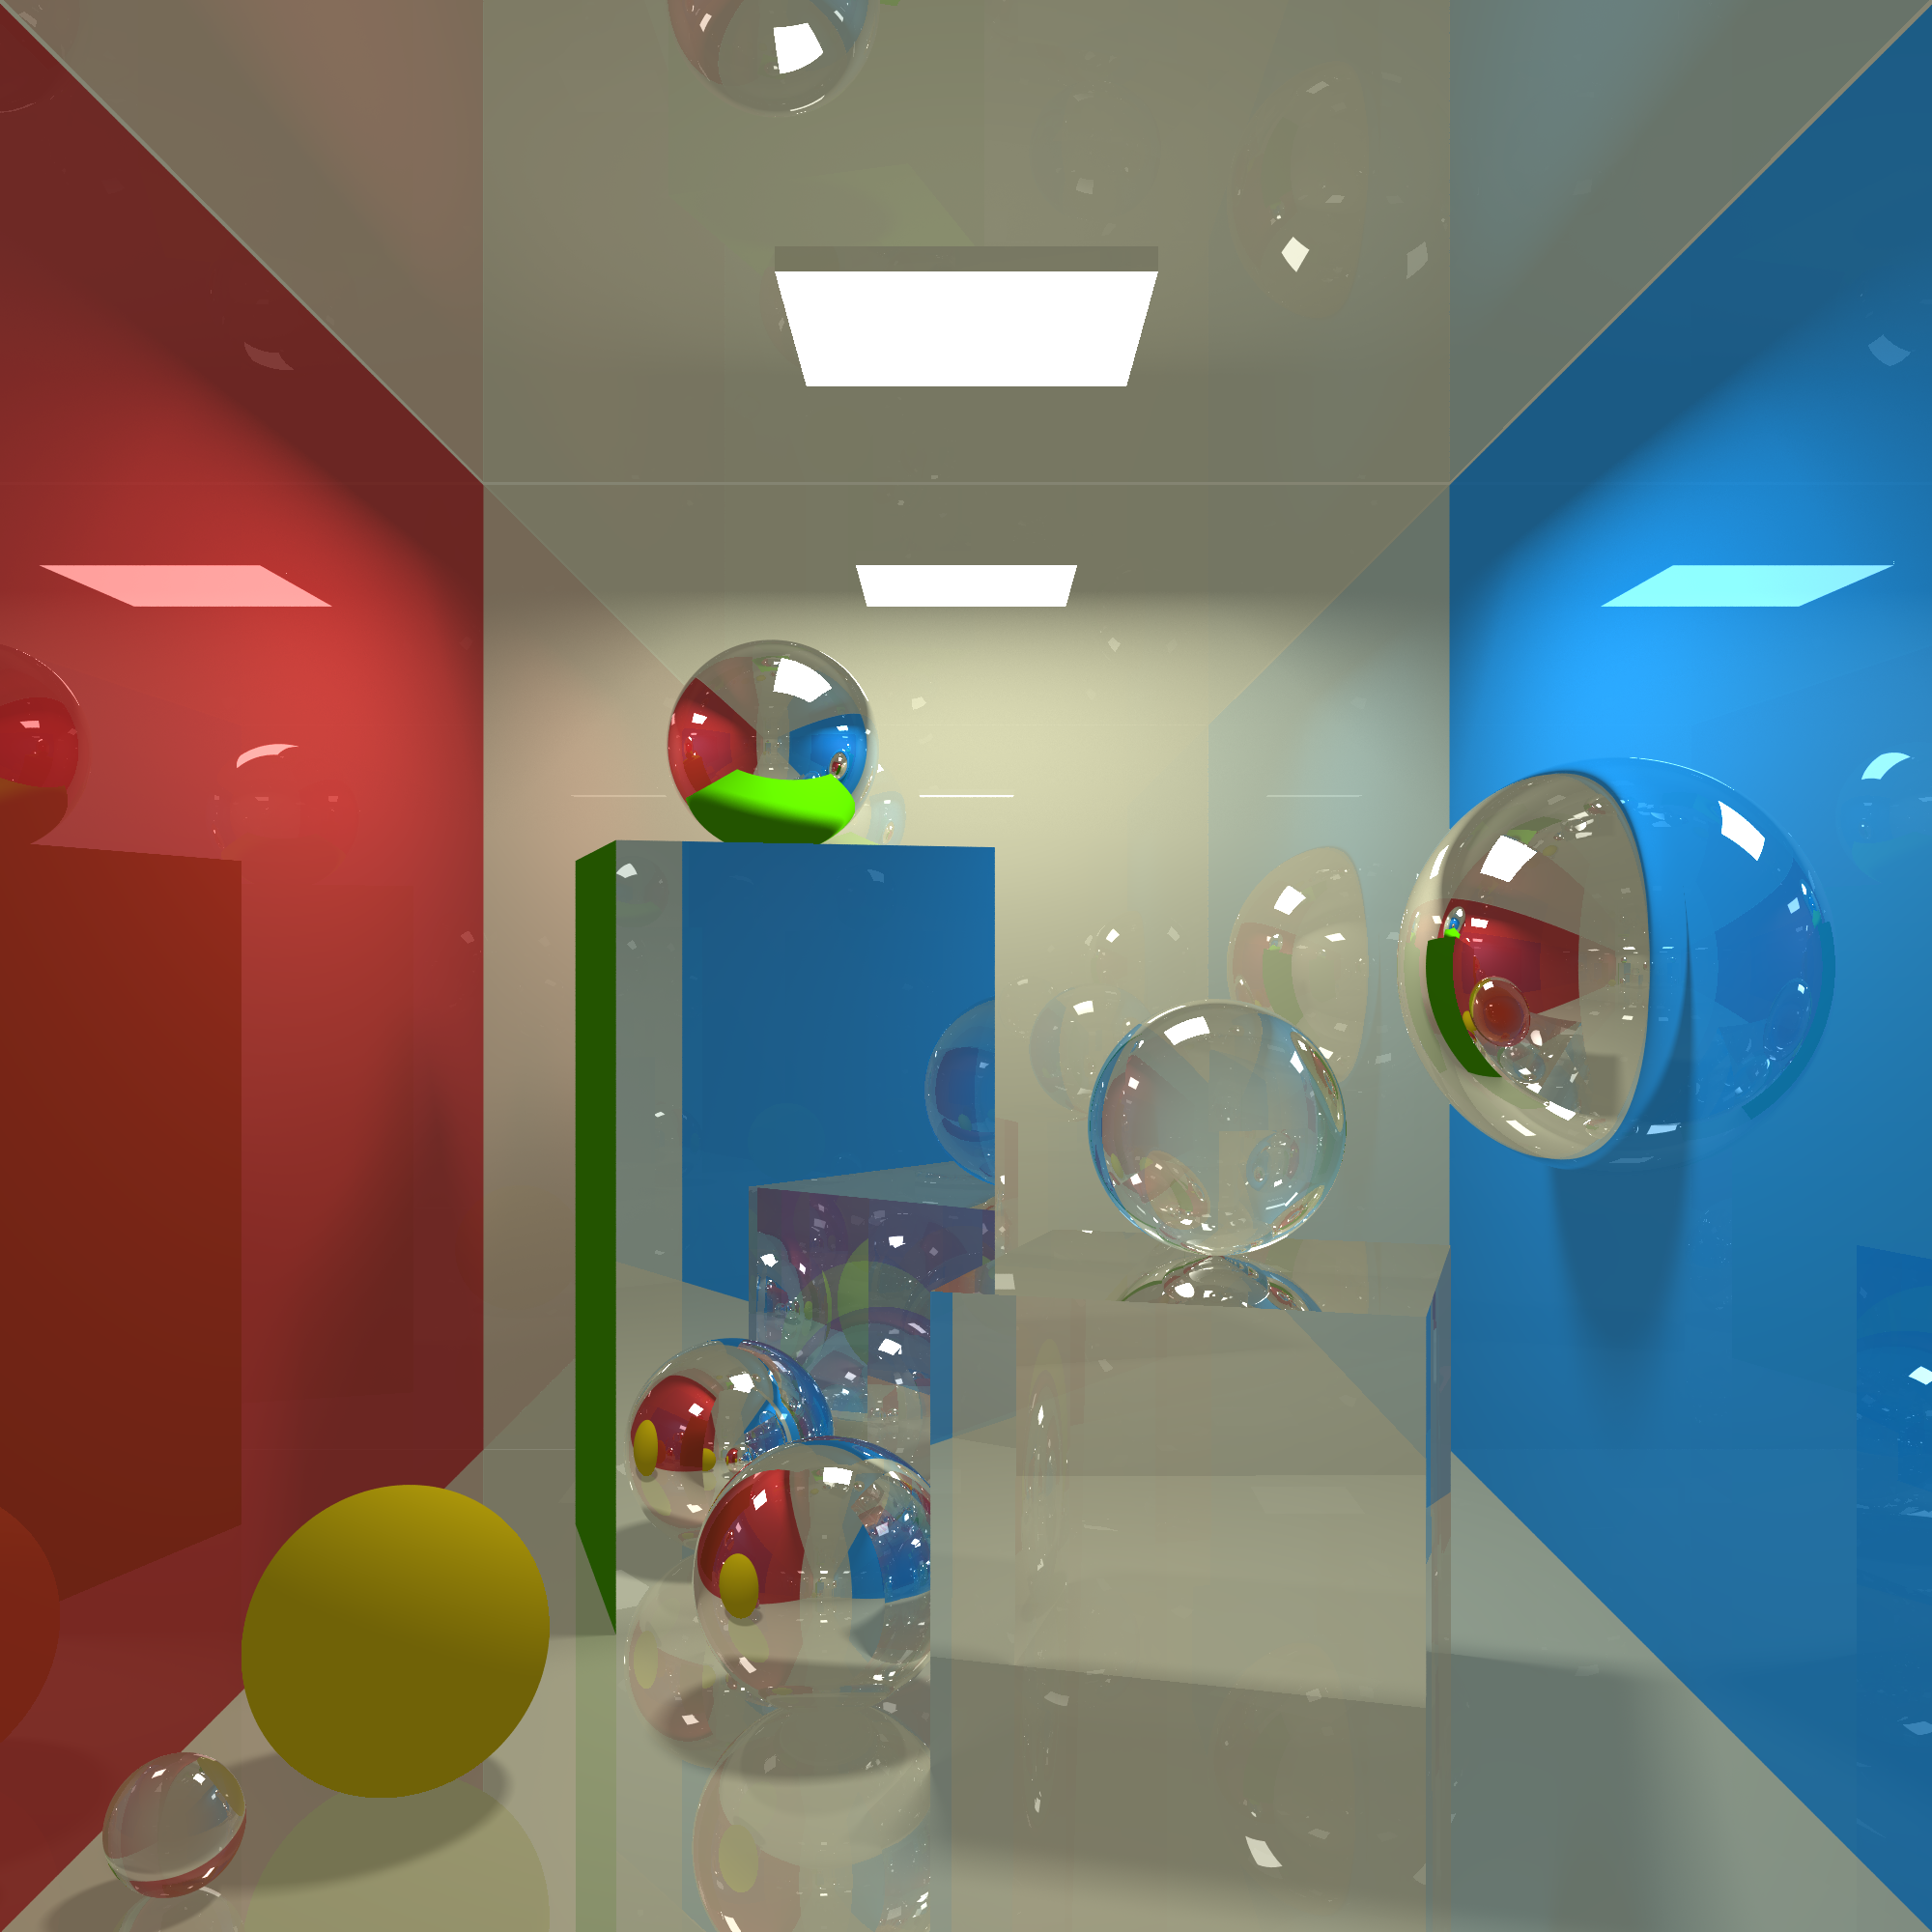
\includegraphics[width=0.35\linewidth]{img/final.png}
%\caption{Final scene}
%\end{figure}
